
%(BEGIN_QUESTION)
% Copyright 2007, Tony R. Kuphaldt, released under the Creative Commons Attribution License (v 1.0)
% This means you may do almost anything with this work of mine, so long as you give me proper credit

The {\it Orbiting Astronomical Observatory} was a NASA project during the late 1960's and 1970's to place precision observational instruments in earth orbit for scientific purposes.  Satellites designed for this program had to have ``hardened'' circuitry to withstand the radiation, extreme temperatures, and other harsh conditions of space.

An example of some of this ``fail-safe'' circuitry is shown here: a passive, quad-redundant, two-input AND gate:

$$\includegraphics[width=15.5cm]{i02514x01.eps}$$

Determine how many component failures this circuit is able to tolerate and still be guaranteed to work.  Specify whether the tolerable faults are {\it opens} or {\it shorts}.

\vfil

\underbar{file i02514}
\eject
%(END_QUESTION)





%(BEGIN_ANSWER)

This is a graded question -- no answers or hints given!

%(END_ANSWER)





%(BEGIN_NOTES)

Tolerable faults for this circuit:

\begin{itemize}
\item{} Resistor ``open'' failures: {\it as many as three resistors failed}
\item{} Resistor ``shorted'' failures: {\it none}
\item{} Diode ``open'' failures: {\it one diode failed, possibly two depending on which two fail}
\item{} Diode ``shorted'' failures: {\it one diode failed, possibly two depending on which two fail}
\end{itemize}

The fact that this circuit design could not tolerate any shorted resistors is not as big a problem as you might think, because resistor shorts are {\it extremely} unlikely.  Usually when we consider the chance that a resistor might be shorted, we are actually considering the chance that a solder bridge lies across the resistor terminals on the circuit board -- a manufacturing defect.  Since all of these NASA circuits were extensively tested before installation in the satellite, no such soldering defects would have actually made their way to the satellite.  Therefore, the extremely remote possibility of a resistor actually failing shorted within itself was of negligible concern.

%INDEX% Safety, redundancy: analog voting

%(END_NOTES)


